\chapter{Friction, Diffusion and the Dissipative Vortex}\label{ch07}
\raggedbottom% this chapter has long unbreakable code boxes and floats: let a page end short rather than stretch the glue; restored at the end of the chapter
\edef\chsevenwp{\the\widowpenalty}\edef\chsevencp{\the\clubpenalty}\widowpenalty=10000 \clubpenalty=10000 % no widows or orphans in this chapter; restored at its end

\section{A pair that opens, a pair that closes}\label{ch07:intro}

In an oblate sodium condensate two vortices of the same sign circle each other, and the pair is seen to open up: its separation grows with time, and grows faster in a warmer
cloud~\cite{Moon2015}. Read through a dissipative point-vortex model, the opening rate is a friction coefficient $\alpha$ between $0.01$ and $0.03$ over the
$200$--$450$~nK explored. In a rubidium condensate in a hard-walled optical trap, a crystal of vortices placed by optical tweezers and then released expands for the same reason;
fitting the expansion to a scaling law gives $\alpha=3.3(1)\times10^{-3}$, while the random wandering of the same vortices is about a hundred times larger than the theory that ties
it to the friction predicts, a surplus that the authors consider most likely due to vibrations of the trap walls~\cite{Neely2024}. Two things are read from the motion of a vortex: how
hard it is dragged, and how hard it is kicked.

Both come from one fact: a vortex in a warm superfluid is not alone. Around it is a gas of thermal excitations, the normal component of Landau's two-fluid
description~\cite{Landau1941}, and the vortex and the gas exchange momentum, which is called \emph{mutual friction}~\cite{Donnelly1991,Sergeev2023}. The gas acts on the vortex with a force along
its velocity relative to the gas and a force across it, and, when the gas is also the heat bath of the vortex, a third effect, random kicks, has to be added: three numbers, $\alpha$, $\alpha'$ and
$\eta$ (\cref{ch07:model}). This chapter follows the model through the three instruments of the book, in a classical field that has no walls, no reservoir and no noise put in by hand, so that the bath
of a vortex is the field's own thermal phonons.

The programme's record on these questions is mixed, and it is told as it stands in the ledger. What survives: the friction of a vortex pair in the field, $\alpha=0.0062(4)$ at
$T/T_{\rm BKT}=0.14$, read by two independent estimators, and a transverse coefficient that is zero to about one per cent. What the programme's own pre-registered tests refuted: the reading of
the friction as proportional to the normal density with a coefficient that belongs to the vortex; the explanation of a stalled single pair by the phonon wind of a closed box; and, earlier, a
known-answer gate that had seemed to pass on a defective instrument. What the decision rule written before the data leaves undecided: the Einstein relation between diffusion and friction.
And one finding is a bias in the very estimator that Lean proves exact in the model: a lesson about hypotheses, not about Lean.

\section{The dissipative point vortex}\label{ch07:model}

Work in units $\hbar=m=1$, so that the circulation quantum is $\kappa=2\pi$, in the frame where the normal component is at rest. A vortex of charge $q=\pm1$ is carried by the superfluid
velocity $\mathbf v_s$ that the other vortices induce at its position; the gas adds a drag along the velocity of the vortex relative to the gas and a force across it. In the two-fluid
equations of Hall, Vinen, Bekharevich and Khalatnikov these are the coefficients $\alpha$ and $\alpha'$~\cite{Shukla2014}, and for a weakly damped vortex they give
\begin{equation}
  \dot{\mathbf r}_i=(1-\alpha')\,\mathbf v_{s,i}-\alpha\,q_i\,\hat{\mathbf z}\times\mathbf v_{s,i}.
  \label{ch07:eq-motion}
\end{equation}
The second term is perpendicular to $\mathbf v_s$ and \emph{dissipative}: it carries energy from the vortices to the gas, and $\alpha$ is the friction. The factor $1-\alpha'$ only rescales the speed with which the
vortex follows the superfluid and dissipates nothing.

The structure of~\eqref{ch07:eq-motion} is clearest in terms of an energy. For point vortices on the plane $H=-\sum_{i<j}q_iq_j\ln r_{ij}^2$ (on the periodic box of the simulations, $\ln r^2$ is
replaced by the Weiss--McWilliams periodic Green function~\cite{WeissMcWilliams1991}; nothing below depends on it), and $\mathbf v_{s,i}=-\tfrac12 q_i\,\hat{\mathbf z}\times\nabla_iH$. Since $q_i^2=1$,
the friction term is $-\tfrac{\alpha}{2}\nabla_iH$, and the whole configuration obeys
\begin{equation}
  \dot{\mathbf r}\;=\;A(\nabla H)\;-\;\tfrac{\alpha}{2}\,\nabla H,
  \qquad \langle \mathbf v,A\mathbf v\rangle=0\ \text{ for every }\mathbf v,
  \label{ch07:eq-flow}
\end{equation}
a skew part $A$, which contains $\alpha'$ and moves the vortices along level sets of $H$, plus a gradient flow that moves them down $H$. Friction therefore pushes the members of an
opposite-sign pair together, because their energy $\ln d^2$ grows with the separation $d$, and pushes the members of a same-sign pair apart, because their energy $-\ln d^2$ falls as $d$ grows: the
first is the dipole that shrinks in the computer, the second the pair that opens in the sodium cloud.

\begin{keybox}[Three numbers describe a vortex in a warm fluid]
\textbf{$\alpha$} (friction): the vortex is dragged and energy flows from the vortices to the gas. \textbf{$\alpha'$} (transverse coefficient): the gas pushes the vortex sideways, without dissipation.
\textbf{$\eta$} (diffusion): the vortex is also kicked at random, $\langle|\Delta\mathbf r|^2\rangle=4\eta t$. If the gas is the heat bath of the vortex, an Einstein relation
$\eta=\alpha T/(2\pi\rho)$ ($k_B=1$) ties the last to the first.
\end{keybox}

\paragraph{The sideways force.} Thouless, Ao and Niu derived the total non-dissipative transverse force on a vortex as the Magnus force proportional to the superfluid density, the core states not changing
it~\cite{ThoulessAoNiu1996}: the normal fluid exerts no extra sideways force and $\alpha'=0$. Iordanskii~\cite{Iordanskii1964} and later Sonin~\cite{Sonin1997} find a transverse force from
the scattering of thermal excitations, which the programme registered as $\alpha'=\rho_n/\rho$.

\paragraph{The random kicks.} Add independent white noise of diffusion constant $\eta$ to~\eqref{ch07:eq-motion}. Mehdi, Hope, Szigeti and Bradley derive $\eta=\alpha k_BT/(2\pi\hbar\rho_0)$
($\rho_0$ the two-dimensional number density) from a stochastic projected Gross--Pitaevskii theory and single out its measurement as an important test of stochastic point-vortex theory~\cite{Mehdi2023}.
A model of this form had been used for helium films by Ambegaokar, Halperin, Nelson and Siggia, with the noise motivated by fluctuation--dissipation arguments and not derived~\cite{AHNS1980}.

\begin{godfrinbox}{the excitations are the bath}
Phys.\ Rev.\ B \textbf{103}, 104516 (2021) reports inelastic neutron scattering on superfluid $^4$He at the ILL spectrometer IN5: the dispersion relation of the Landau elementary excitations, phonon, maxon and roton, and the thermodynamic
consequences~\cite{Godfrin2021}. Those excitations are the normal component of Landau's picture~\cite{Landau1941}, and in the kinetic theory of mutual friction the friction on a vortex is their scattering by the vortex~\cite{Sergeev2023}. What such a measurement fixes, for helium, is
what sets the scale of every number below: the energy $\varepsilon(k)$ of a thermal excitation, hence the population of the bath. In our classical field the model must supply the bath itself, and \cref{ch07:law} shows how little it resembles a quantum gas. The statements of his papers that the library formalises are in \cref{ch04,ch05}, not here.
\end{godfrinbox}

\section{What Lean proves about the model}\label{ch07:lean}

Three modules of the library concern this chapter, \lean{Dissipative\-Vortex\-Dynamics}, \lean{Einstein\-Relation} and \lean{Friction\-Kinetic} (a fourth, \lean{QuasiPeriodic\-Bound}, appears once); a small new module written for the book adds statements to the first. The
mathematics is elementary calculus, and the modules say so. The point is that the estimators used on the data are \emph{identities of the model}, with the hypotheses under which they
hold written where a machine can read them. Every theorem quoted here depends only on the three standard axioms \texttt{propext}, \texttt{Classical.choice} and \texttt{Quot.sound}: the library modules carry no
\texttt{\#print axioms} lines, so this was checked on 2026-10-09 by compiling scratch copies with one such line per theorem (Lean~4.34.0-rc2, the pinned Mathlib; no errors, no \texttt{sorry}).

The first theorem is general: any dynamics of the form~\eqref{ch07:eq-flow}, on any real inner-product space (any number of vortices, plane or torus), with $A$ pointwise skew.

\begin{leanbox}[unbreakable]{DissipativeVortexDynamics}
\begin{lstlisting}[style=lean,basicstyle=\ttfamily\footnotesize]
variable {X : Type*} [NormedAddCommGroup X] [InnerProductSpace ℝ X] [CompleteSpace X]
theorem energy_dissipation (H : X → ℝ) (gradH : X → X) (hH : ∀ x, HasGradientAt H (gradH x) x)
    (A : X → X) (hA : ∀ v, inner ℝ v (A v) = 0) (γ : ℝ) (r : ℝ → X)
    (hr : ∀ t, HasDerivAt r (A (gradH (r t)) - γ • gradH (r t)) t) (t : ℝ) :
    HasDerivAt (fun t => H (r t)) (-γ * ‖gradH (r t)‖ ^ 2) t := by
\end{lstlisting}
\nopagebreak[4]\smallskip\noindent\textit{(Proof abridged: eleven lines in the module, the chain rule and then \texttt{hA}.)}
\end{leanbox}

In words: along any solution, $\frac{d}{dt}H=-\gamma\|\nabla H\|^2$, \emph{whatever the skew part}. For~\eqref{ch07:eq-motion}, $\gamma=\alpha/2$ and $\|\nabla H\|^2=4\sum_i|\mathbf v_{s,i}|^2$, hence
\begin{equation}
  \frac{dH}{dt}=-2\alpha\sum_i|\mathbf v_{s,i}|^2,\qquad
  \alpha_{\rm energy}=-\frac{\Delta H}{2\int\sum_i|\mathbf v_{s,i}|^2\,dt}.
  \label{ch07:eq-energy}
\end{equation}
The right-hand side estimates $\alpha$ from the positions of the tracked vortices alone, needs no pairing of them, and is blind to $\alpha'$ (\Lthm{DissipativeVortexDynamics}{dissipation_indep_of_skew}). This is the programme's
\emph{energy estimator}. Its hypothesis, written in the statement, is \texttt{hr}: the path has a derivative at every time. We shall come back to it.

For the plane dipole the model can be written in coordinates. Let $\mathbf p$ be the $+$ vortex, $\mathbf m$ the $-$ vortex, $\mathbf d=\mathbf p-\mathbf m$ and $\texttt{r2}=|\mathbf d|^2$; the superfluid velocity at either vortex is $(d_y,-d_x)/\texttt{r2}$.
The hypotheses \texttt{hpx}, \texttt{hpy}, \texttt{hmx}, \texttt{hmy} below are the model~\eqref{ch07:eq-motion} for the two vortices, and \texttt{hpos} says $\texttt{r2}\neq0$.

\begin{leanbox}[unbreakable]{DissipativeVortexDynamics}
\begin{lstlisting}[style=lean,basicstyle=\ttfamily\footnotesize]
variable (px py mx my : ℝ → ℝ) (α α' : ℝ)

/-- squared separation -/
noncomputable def r2 (t : ℝ) : ℝ := (px t - mx t) ^ 2 + (py t - my t) ^ 2

include hpx hpy hmx hmy hpos

theorem dipole_sq_law (t : ℝ) (ht : t ∈ Icc (0 : ℝ) T) :
    r2 px py mx my t = r2 px py mx my 0 - 4 * α * t := by

theorem centre_velocity_identity (t : ℝ) (ht : t ∈ Icc (0 : ℝ) T) :
    ∃ cx' cy' : ℝ, HasDerivAt (fun s => (px s + mx s) / 2) cx' t ∧ HasDerivAt (fun s => (py s + my s) / 2) cy' t ∧
      cx' * (py t - my t) - cy' * (px t - mx t) = 1 - α' ∧
      cx' * (px t - mx t) + cy' * (py t - my t) = 0 ∧
      (cx' ^ 2 + cy' ^ 2) * r2 px py mx my t = (1 - α') ^ 2 := by
\end{lstlisting}
\nopagebreak[4]\smallskip\noindent\textit{Statements only (the four hypotheses are lines 88--96 of the module); the proofs are in the module.}
\end{leanbox}

First, $|\mathbf d|^2=|\mathbf d_0|^2-4\alpha t$ for as long as the pair exists, \emph{whatever $\alpha'$}: a dipole is a clock whose dial is $|\mathbf d|^2$, calibrated in units of $4\alpha$, with a lifetime below
$|\mathbf d_0|^2/4\alpha$. The proof is the computation $\frac{d}{dt}|\mathbf d|^2=-4\alpha$ and the fact that a function with vanishing derivative on an interval is constant (the theorems
\Lthm{DissipativeVortexDynamics}{r2_hasDerivAt} and \Lthm{DissipativeVortexDynamics}{dipole_lifetime_bound} are the two steps). Second, the centre of the pair moves perpendicular to its axis at speed $(1-\alpha')/|\mathbf d|$, whatever $\alpha$. The shrinking of the pair measures $\alpha$, its
translation measures $\alpha'$, and the two are read from orthogonal observables.

\subsection*{A same-sign pair: new Lean}

The simulations of this chapter imprint dipoles; the experiment that opened it watched the other pair, two vortices of the \emph{same} sign. The book's new module \lean{Ch07\_DissipativePairs}
(in \texttt{book/lean/}, not part of the library) proves the corresponding law with the same method: for $\mathbf d=\mathbf p_1-\mathbf p_2$ the model gives
$\dot{\mathbf d}=[\,2(1-\alpha')\,\hat{\mathbf z}\times\mathbf d+2\alpha\,\mathbf d\,]/|\mathbf d|^2$, so $\frac{d}{dt}|\mathbf d|^2=+4\alpha$.

\begin{leanbox}{Ch07\_DissipativePairs (new, not in the library)}
\begin{lstlisting}[style=lean,basicstyle=\ttfamily\footnotesize]
theorem corot_sq_law (t : ℝ) (ht : t ∈ Icc (0 : ℝ) T) :
    r2 x1 y1 x2 y2 t = r2 x1 y1 x2 y2 0 + 4 * α * t := by
\end{lstlisting}
\nopagebreak[4]\smallskip\noindent\textit{Statement only; the hypotheses are the four equations of the model for two charges of equal sign (lines 41--51 of the file), the proof is that of the dipole law above. The file compiled on 2026-10-09 with no error and no \texttt{sorry}, and the theorem uses only the three standard axioms.}
\end{leanbox}

Friction makes opposite-sign pairs shrink and same-sign pairs spiral apart; the new theorem formalises a derivation, not a result about any fluid.

\section{The model in CVODE}\label{ch07:cvode}

The point-vortex equations are smooth, small and not stiff until a pair is a few core sizes across, and they have closed forms: the right first test of an integrator, and a way of seeing what the theorems say. CVODE~\cite{Hindmarsh2005} is reached from
Python through \texttt{rusty\_sundials.CvodeSolver(method, rtol, atol, max\_steps)}, whose method \texttt{solve(rhs, t0, y0, t\_out)} returns the state at \texttt{t\_out} (\cref{ch02}); the binding builds a fresh solver at every call, so a table of outputs is a chain of calls.

\Cref{ch07:fig-dipole}, computed with the listing below, puts CVODE next to the theorems. Panel~c is \Lthm{DissipativeVortexDynamics}{dipole_sq_law} and \Lthm{DissipativePairs}{corot_sq_law} as measured: with BDF at relative tolerance $10^{-8}$ the largest relative
deviation of $|\mathbf d|^2$ from the law over $0.95$ of the lifetime is between $1.8\times10^{-8}$ and $2.9\times10^{-8}$ for the six combinations of $\alpha$ and $\alpha'$ (dipoles) and $4.6\times10^{-6}$ to $1.1\times10^{-5}$ for the same-sign pairs, which turn about ten times (an integrator conserves nothing, and the error of a rotating pair accumulates over its turns); the slope does not depend on $\alpha'$.
Panel~d: the displacement of the centre follows the closed form (the integral of the centre identity, done by hand; it is not a Lean theorem) to $2.1\times10^{-5}$ over a track of length $311$.

Panel~e is the solver's side of the same coin. On this non-stiff problem Adams needs between a quarter and a third of the work of BDF at the same tolerance in a single call (93--372 right-hand-side evaluations over the four tolerances, against 413--1198); the chain of $60$ outputs that a figure needs costs 7 to 21 times more, because the method restarts at low order at every call, and its error is not monotone in the tolerance (for BDF $1.2\times10^{-5}$ at $10^{-4}$ and $1.1\times10^{-5}$ at $10^{-6}$).
These numbers are for the build of rusty-SUNDIALS at commit \texttt{5db8041} (six commits after v11.5.0), not for the module installed in the shared virtual environment, whose Adams method is the one before the repository's fix: on $y'=-y$ up to $t=10$ at $\texttt{rtol}=10^{-8}$ the stale module needed 237\,022 right-hand-side evaluations and the fixed build 511. The figure script runs this probe first and refuses the stale module.

\begin{rustbox}[unbreakable]{the dissipative dipole in CVODE}
\begin{lstlisting}[style=py,basicstyle=\ttfamily\footnotesize]
def rhs_dipole(a, ap):
    def rhs(t, y):
        px, py, mx, my = y; dx = px - mx; dy = py - my; r2 = dx * dx + dy * dy
        return [((1 - ap) * dy - a * dx) / r2, (-(1 - ap) * dx - a * dy) / r2,
                ((1 - ap) * dy + a * dx) / r2, (-(1 - ap) * dx + a * dy) / r2]
    return rhs
# ...
def integrate(rhs, y0, tgrid, rtol, atol=1e-10, method="bdf"):
    s = CvodeSolver(method=method, rtol=rtol, atol=atol, max_steps=200000)
    t = float(tgrid[0]); y = list(y0); out = [list(y)]
    for tn in tgrid[1:]:
        t, y = s.solve(rhs, t, y, float(tn)); out.append(list(y))
    return np.array(out)
\end{lstlisting}
\nopagebreak[4]\smallskip\noindent\textit{Excerpt of \texttt{book/figures/ch07\_dipole.py}, as run (\texttt{rhs\_corot} is its mirror image for two $+$ vortices). The figure took 2.5\,s of wall-clock on the shared 8-core machine (load average $3.5$--$3.8$), with rusty-SUNDIALS commit \texttt{5db8041} (see below).}
\end{rustbox}

\begin{figure}[!tb]\centering
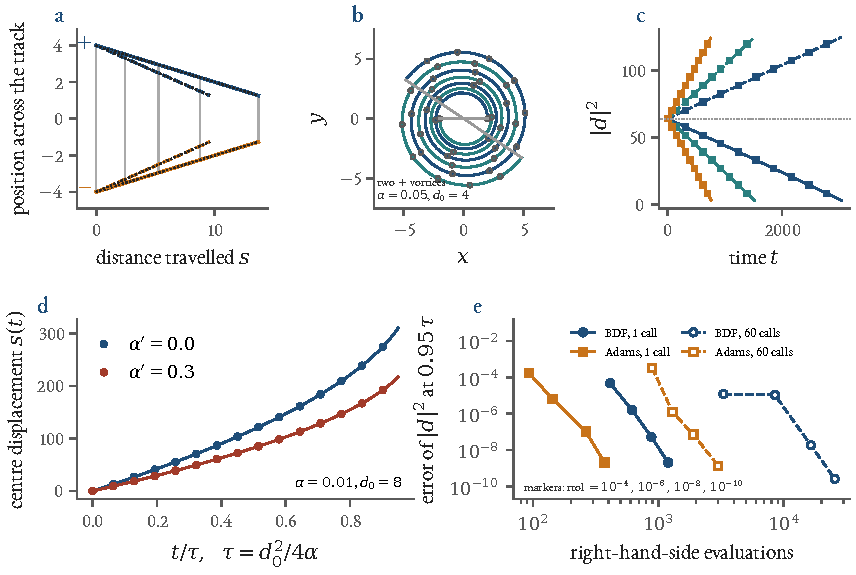
\includegraphics[width=\linewidth]{figures/ch07_dipole.pdf}
\caption[CVODE against the Lean statements on dissipative vortex pairs]{CVODE (\texttt{rusty\_sundials}) against the statements of \cref{ch07:lean}. \textbf{a}~A dipole shrinking and translating: $+$ (blue) and $-$ (orange) vortices in the frame of the track, $\alpha'=0$ (solid) and $0.3$ (dashed),
exact curves dotted, pair axis in grey at five times; $\alpha=0.2$ is ten times a thermal value, chosen so that the funnel is visible. \textbf{b}~Two $+$ vortices spiral apart ($\alpha=0.05$, $d_0=4$, $600$ time units, 3.4 turns);
grey circles: closed form. \textbf{c}~$|\mathbf d|^2$ against time: dipoles (solid) fall with slope $-4\alpha$, same-sign pairs (dashed) rise with $+4\alpha$, for $\alpha=0.005,\,0.01,\,0.02$ (blue, teal, orange); filled markers $\alpha'=0$, open $\alpha'=0.3$.
\textbf{d}~Displacement of the centre of a dipole against the closed form $s=(1-\alpha')(d_0-d)/2\alpha$. \textbf{e}~Work and precision: right-hand-side evaluations against the error of $|\mathbf d|^2$ at $0.95$ of the lifetime ($\alpha=0.01$, $\alpha'=0.1$) for BDF and Adams at $\texttt{rtol}=10^{-4},\dots,10^{-10}$, in one call (filled) and in a chain of $60$ outputs (open).}
\label{ch07:fig-dipole}
\end{figure}


\section{A vortex pair in a thermal field}\label{ch07:field}

\subsection*{The instrument}

The field is the projected Gross--Pitaevskii equation $i\partial_t\psi=\mathcal P[-\tfrac12\nabla^2\psi+g|\psi|^2\psi]$ on a periodic square box of side $L=64$, with $\hbar=m=g=1$ and mean density $n=1$ (healing length $\xi=1$, sound speed $c=1$),
$128\times128$ grid points and a sharp cutoff $|k|\le k_c=\pi$, half the grid wavenumber~\cite{Davis2001,Blakie2008}. The energy is conserved (to $10^{-7}$--$10^{-6}$ over every run of the campaign); nothing is damped and no noise is added. The temperature of a
base state comes from an equipartition thermometer and its normal fraction from the current correlators~\cite{Callens2026a}. The base state of this section is the campaign's $e=0.60$ state: $T=0.115$, that is $T/T_{\rm BKT}=0.14$ with $T_{\rm BKT}(L{=}64)=0.821$ from a heating
ladder, and $\rho_n/\rho=0.027$.

A pair is written into the state by multiplying $\psi$ by the Jacobi-theta phase of the vortex configuration, made single-valued on the torus by a uniform phase gradient, and by the Bernoulli amplitude $[1+|\mathbf v|^2/2]^{-1/2}$ of the imprinted flow. Vortices are found by the
plaquette phase-winding rule that \lean{VortexWinding} proves correct (\cref{ch03}), refined to sub-grid precision, followed by continuity (same sign, nearest detection within $3\xi$) and recorded every time unit. A single pair in a periodic box carries impulse and drives a mean flow, so the
simulations imprint \emph{two antiparallel pairs}, a $+-$ pair at $x=L/4$ and a $-+$ pair at $x=3L/4$ of equal separation $d_0$: zero net charge, dipole moment and impulse, the two pairs travelling in opposite directions.

\begin{rustbox}{two antiparallel pairs in a thermal field (qf-pgpe)}
\begin{lstlisting}[style=py,basicstyle=\ttfamily\footnotesize]
c = np.ascontiguousarray(s.imprint_v2(np.ascontiguousarray(c0), pos, q)); E0 = s.energy(c); t = 0.0; last = pos.copy()
# ...
dp, dq = s.detect(c); dp = np.asarray(dp); dq = np.asarray(dq); cur = np.full_like(last, np.nan)
for i in range(len(q)):
    cand = np.nonzero(dq == q[i])[0]
    if len(cand):
        d = dp[cand] - last[i]; d -= L * np.round(d / L); r = np.hypot(d[:, 0], d[:, 1]); j = int(np.argmin(r))
        if r[j] <= a.r_track:
            cur[i] = dp[cand[j]]
# ...
c = np.ascontiguousarray(s.run(c, 1.0)); t += 1.0
\end{lstlisting}
\nopagebreak[4]\smallskip\noindent\textit{Excerpt of \texttt{book/figures/ch07\_pairrun.py}, as run (\texttt{s} is \texttt{qf\_pgpe.Pgpe(128, 64.0)}, \texttt{c} the projected Fourier amplitudes, \texttt{last} the previous positions). The run was advanced in five chunks of $100$ to $500$ time units, each under the
shared-machine lock, and checkpointed: 928\,s of wall-clock for 1500 time units on one thread, at load average $7$--$18$ on 8 cores.}
\end{rustbox}

\subsection*{The control that caught the first instrument}

An instrument has to be tested where the answer is known. At $T=0$ a pair in a uniform condensate has no excitation to rub against, and the model says its separation must not shrink. The campaign's first known-answer gate did not use this control: it was a single dipole at $T/T_{\rm BKT}\approx0.14$ with the
imprint of the earlier rounds and a biased vortex detector, and it \emph{passed}, narrowly: four fits gave $\alpha=0.0093,\ 0.0062$ ($d_0=8$) and $0.0028,\ 0.0022$ ($d_0=12$), median $0.0045$, inside the window $[0.004,0.045]$ registered from an interpolation of the values published by Shukla, Brachet and Pandit~\cite{Shukla2014}.
That the friction fell with the size of the pair was not predicted, and was noted. The $T=0$ control was run next, and it failed.

\begin{figure}[!tb]\centering
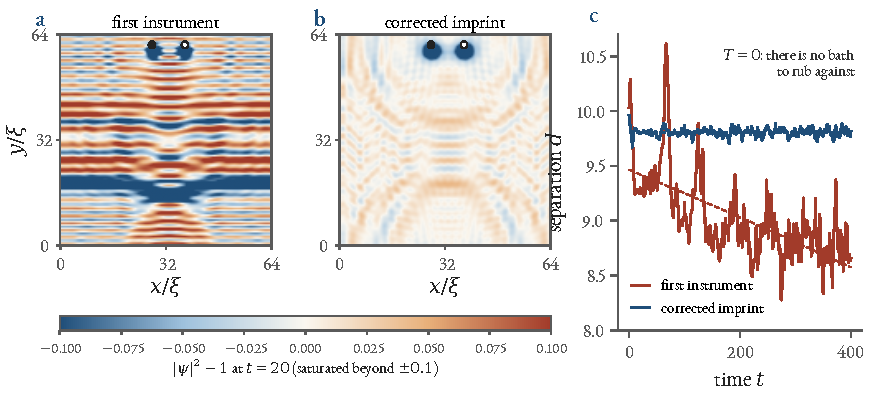
\includegraphics[width=\linewidth]{figures/ch07_imprint.pdf}
\caption[A zero-temperature control of the vortex imprint]{A $T=0$ control. A single pair of separation $10$ is imprinted in a uniform condensate ($L=64$) and $|\psi|^2-1$ is shown $20$ time units later. \textbf{a}~The imprint of the first instrument leaves a phase step along a whole line of the box and a density tail, which become a sheet of sound.
\textbf{b}~The corrected imprint leaves a quiet wake. \textbf{c}~Separation against time over $400$ time units, from the archived tracks of the two gate runs (first attempt: failed; second: passed); dashed, a straight line fitted to $d^2$.}
\label{ch07:fig-imprint}
\end{figure}

\Cref{ch07:fig-imprint} shows why. With the first imprint the pair, which cannot lose energy to a bath that does not exist, closed from $10.03$ to $8.66$ in $400$ time units: an \emph{apparent} friction $\alpha=0.0100$ from the slope of $d^2$, more than the thermal value measured later at $T/T_{\rm BKT}=0.14$ ($0.0062$).
The peak density just after the imprint is $1.084$ against $1.007$ with the corrected one, and at $t=20$ the field momentum is $0.75$ of $2\pi nd$ against $0.96$. Two defects were responsible: the theta-function phase of a single pair is periodic on the torus only if
$\sum_iq_i\mathbf r_i\in L\mathbb Z^2$, otherwise it jumps by $2\pi d/L$ across a boundary and the projection turns the jump into a sheet of sound; and the usual per-vortex amplitude $[r^2/(r^2+2)]^{1/2}$ has a $1/r^2$ tail four times the Bernoulli depletion, whose excess leaves as sound and pushes the vortices (cf.~\cite{Rorai2013}).
With the corrected imprint the pair stays at $9.96\to9.81$ ($|\alpha_{\rm apparent}|<10^{-5}$).

The ledger records the consequence without softening: the pass of the first gate \emph{is withdrawn}, and the stalled single pair that had motivated the hypothesis of \cref{ch07:wind} lost its standing as evidence. The replacement is the corrected instrument at $T=0.115$ with a window fixed in advance: $\alpha_{\rm energy}=0.00705\pm0.00012$ in $[0.0028,0.0112]$.
The lesson is which known answer to ask for first: the $T=0$ control is the cheapest, and the one a theorem makes decisive, since with no bath there is nothing to dissipate into.

\subsection*{The field, and what is measured in it}

\begin{figure}[!tb]\centering
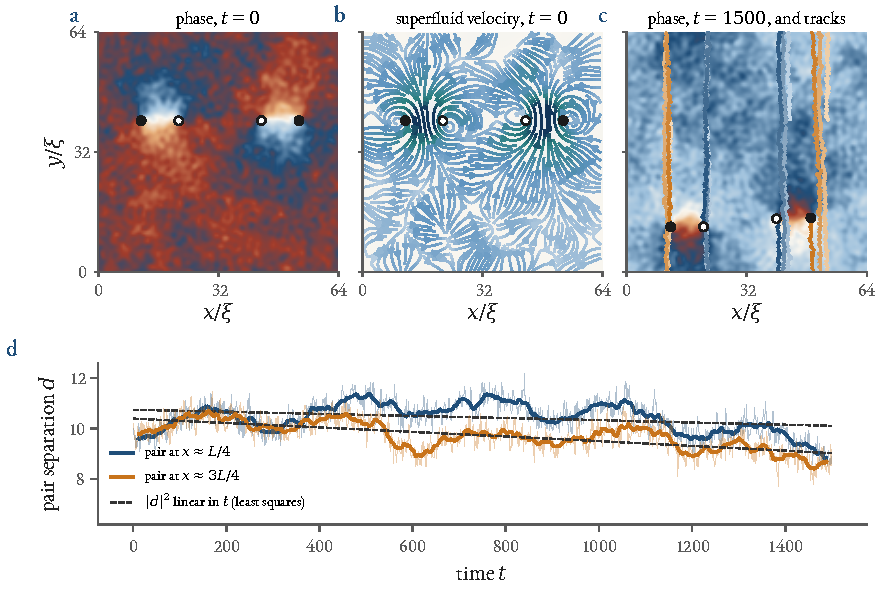
\includegraphics[width=\linewidth]{figures/ch07_fields.pdf}
\caption[Two antiparallel vortex pairs in a thermal projected Gross--Pitaevskii field]{Two antiparallel vortex pairs in a thermal projected-GP field ($T=0.115$, $T/T_{\rm BKT}=0.14$, $L=64$, $d_0=10$), evolved with the Rust engine for 1500 time units (one run, seed 7; relative energy drift $6.8\times10^{-8}$).
\textbf{a}~Phase of $\psi$ just after the imprint; open circles are $+$ vortices, filled circles $-$ vortices. \textbf{b}~The superfluid velocity $\mathrm{Im}(\psi^*\nabla\psi)/|\psi|^2$ coarse-grained over $3\xi$: the jets between the members of each pair and the return flow around them;
the thermal phonons are the faint background. \textbf{c}~Phase at the end of the run with the four tracks (colour: time, drawn on the periodic box). \textbf{d}~Separations of the two pairs against time; dashed, least-squares fits of $d^2$ against $t$.}
\label{ch07:fig-fields}
\end{figure}

\Cref{ch07:fig-fields} shows what the instrument sees. At $t=0$ each pair is a dipole: between its members the superfluid velocity is a jet of speed about $1/d$, the two jets point in opposite directions, and each vortex rides on the jet of its partner. Over 1500 time units the two pairs travel about 2.5 times round the box in opposite directions, at the speeds $0.104$ and $0.111$ (the planar $1/d$ would give about $0.1$). The torus point-vortex model, evaluated at the tracked positions, gives $0.102$ and $0.111$: the measured speed is $1.018$ and $0.998$ of the model's, the regression coefficient $1-\alpha'$ below being $1.007\pm0.006$ (jackknife over eight blocks of the track), so that the centre moves at the model velocity with no sideways force within the errors, as the centre identity of \cref{ch07:lean} says it should. (The planar formula $1/d$ is 6 and 7 per cent below the model for the two pairs: the model adds the periodic images and the second pair.) The separations go from 9.7 to 8.8, between 8.4 and 11.4 along the way: the run reached the planned $t=1500$ with all four vortices tracked throughout. The detected position of a core jitters by $0.31$ per coordinate (the zero-lag offset of the residuals, $c_0=0.20$, for the archived runs of this arm).
A least-squares slope of $d^2$ reads $\alpha=0.0033$ (mean of the two pairs; separately $+0.0022$ and $+0.0044$): to be compared with the estimators below, not trusted over them.

The estimators the programme registered are the energy identity~\eqref{ch07:eq-energy} and a two-coefficient regression: for each tracked vortex the displacement over a lag of $10$ time units is regressed on $\int\mathbf v_{s,i}\,dt$ and $-q_i\!\int\hat{\mathbf z}\times\mathbf v_{s,i}\,dt$, with $\mathbf v_{s,i}$ the torus point-vortex velocity induced by the \emph{other tracked vortices}; the
coefficients are $1-\alpha'$ and $\alpha$, and the mean square of the residuals against lag gives $\eta$. Both are in the Rust extension, \texttt{qf\_pgpe.analyse\_tracks(tracks, 64.0)}, which takes a list of (times, positions, charges) and returns the estimates with block-jackknife errors. It agrees with the Python code of the campaign to $1\times10^{-14}$ (relative) on the eight archived tracks
of this arm (Python: 29\,s; Rust: 1.2\,s, on the loaded machine) and reproduces the campaign's numbers: $\alpha_{\rm energy}=0.00617\pm0.00041$, $\alpha_{\rm regression}=0.00645\pm0.00037$, $1-\alpha'=1.0100\pm0.0015$.

\begin{figure}[!tb]\centering
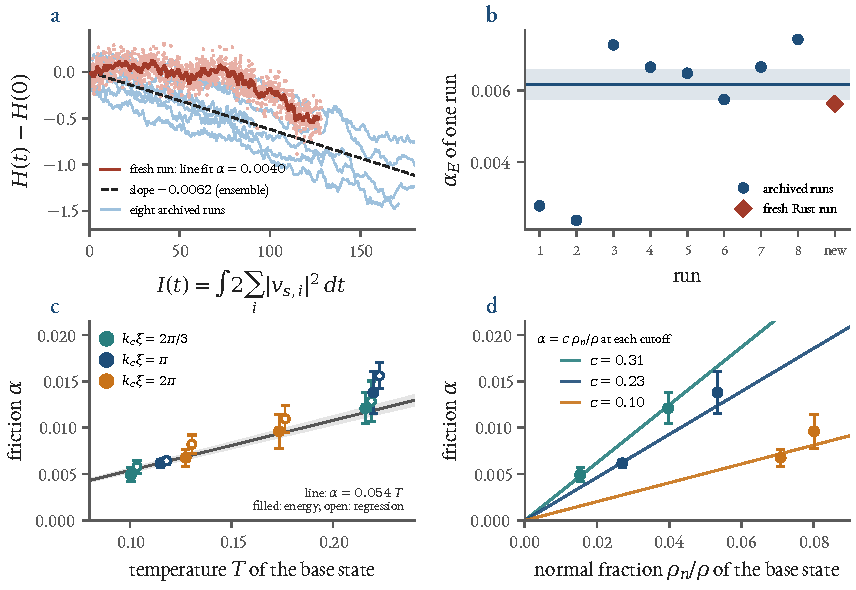
\includegraphics[width=\linewidth]{figures/ch07_friction.pdf}
\caption[The friction in the field]{The friction in the field. \textbf{a}~The energy identity on the tracks: $H(t)-H(0)$ against $I(t)=\int2\sum_i|\mathbf v_{s,i}|^2dt$ falls along a line of slope $-\alpha$ (red: the fresh run, samples and means of $25$ consecutive samples; light blue: the eight archived runs, the same means over the same duration; dashed: the slope of the ensemble).
\textbf{b}~Single-run estimates $\alpha_E$ at $T=0.115$: the eight archived runs and the fresh one, against the ensemble mean and its jackknife error (band). \textbf{c}~The friction of the six arms of the cutoff scan against the temperature of the base state (filled: energy estimator; open, shifted right: regression); the line is
$\alpha=0.054\,T$ (band: one standard error). \textbf{d}~The same data against the normal fraction: within each cutoff the points are proportional to $\rho_n/\rho$, with a coefficient $c$ that changes by a factor $3$ from one cutoff to the next.}
\label{ch07:fig-friction}
\end{figure}

\Cref{ch07:fig-friction}a is the theorem at work, with its caveat. For every run $H(t)$ and $I(t)$ are computed from the tracked positions only, and the identity says that they lie on a line of slope $-\alpha$. The eight archived runs (light blue) do, within the thermal scatter of the detected positions, but with slopes that differ from run to run: over the same
1500 time units their single-run $\alpha_E$ has a mean of $0.0057$ and a standard deviation of $0.0020$, 35 per cent of the mean (panel~b). The fresh run (red) gives $\alpha_E=0.0056$ and $\alpha_R=0.0037$ from the registered estimators (they fit the two halves of every track separately and pool them, so that block-jackknife errors can be given; one straight line through the whole track gives $0.0040$). That puts the run on the ensemble mean (0.02 standard deviations away, number 3 of the nine single runs counted from the lowest).
It is one seed, drawn once and not replaced. The same run analysed at its checkpoint $t=1000$, while the last chunk was waiting for a processor, had given $\alpha_E=-0.0013$ and $\alpha_R=-0.0016$: the estimate of one track moved by $0.0070$ in $500$ time units, and nothing was decided on that interim look.
A pair at this temperature should lose $4\alpha t\approx37$ in $d^2$ over the run, that is, $d$ should fall from $10$ to $7.9$; but the separation of one pair wanders by up to $2.6$ in the $25$-unit means within the run (\cref{ch07:fig-fields}d), so a single track cannot isolate the drift. That is why the campaign used six to eight runs per temperature and quoted jackknife errors over runs; and it is the reason that the identity,
which is exact in the model, is a way of \emph{estimating} $\alpha$ and not a way of seeing it in one track.

\begin{table}[!tb]\centering\small
\begin{tabular}{lcccccc}
\toprule
$T$ & $T/T_{\rm BKT}$ & $\rho_n/\rho$ & runs & $\alpha$ (energy) & $\alpha$ (regression) & $\alpha_{d_0=8}/\alpha_{d_0=12}$\\
\midrule
$0$ & $0$ & $0$ & 1 & $4.1\times10^{-4}$ (floor) & $2.0\times10^{-4}$ & ---\\
$0.115$ & $0.14$ & $0.027$ & $8$ & $0.0062\pm0.0004$ & $0.0064\pm0.0004$ & $0.91$\\
$0.220$ & $0.27$ & $0.053$ & $6$ & $0.0138\pm0.0023$ & $0.0156\pm0.0014$ & $0.76$\\
$0.353^{\dagger}$ & $0.43$ & $0.095$ & $6$ & $0.0205\pm0.0138$ & $0.0242\pm0.0065$ & $1.04$\\
\bottomrule
\end{tabular}
\caption{Friction of a vortex pair in the closed field ($L=64$, $k_c=\pi$; two antiparallel pairs of sizes $8$ and $12$, tracks of up to $2000$ time units), the archived campaign re-analysed with the Rust estimators. Errors are block jackknives over runs.
$^\dagger$A thermal vortex is present in more than $5\%$ of the samples of this base state; the error is large and the base is kept with that flag. The energy estimator is low by the diffusion bias of \cref{ch07:bias}.}
\label{ch07:tab-alpha}
\end{table}

\Cref{ch07:tab-alpha} gives the friction at the three temperatures. The three criteria registered for it passed: the two pair sizes agree (ratios $0.91$, $0.76$, $1.04$, inside the registered $[0.7,1.43]$ at two of three temperatures), $\alpha$ increases with
$T$, and the two estimators agree within $5$, $13$ and $18$ per cent. At $0.14\,T_{\rm BKT}$ the value is a factor two below an interpolation of the values of Shukla, Brachet and Pandit~\cite{Shukla2014}, whose own transition temperature is an estimate; at $0.27$ and $0.43$ no closed-field value existed before, and these lie in the range of the oblate-condensate
measurements~\cite{Moon2015}. One more observation was \emph{not} registered, and is the subject of the next section: $\alpha/(\rho_n/\rho)=0.23,\,0.26,\,0.22$.

\section{Friction follows the temperature, not the normal density}\label{ch07:law}

\subsection*{A kinetic reading, a proportionality, and a prediction}

In the projected field the bath is a finite set of modes $k\in K$ (3208 of them at $k_c=\pi$ in this box). For excitations of occupation $n_k$ and transport cross-section $\sigma_{\rm tr}(k)$ (a length, in two dimensions), a vortex moving slowly through them feels the drag $F=-Dv$ with
$D=\tfrac12\int\frac{d^2k}{(2\pi)^2}(-\partial n/\partial\varepsilon)\,k^2\,c_g\sigma_{\rm tr}$, $c_g=d\varepsilon/dk$, while the Landau normal density of the same gas is $\rho_n=\tfrac12\int\frac{d^2k}{(2\pi)^2}(-\partial n/\partial\varepsilon)\,k^2$: two integrals of the same weight, the first with one extra factor $c_g\sigma_{\rm tr}$.
A force balance on a weakly damped vortex gives $\alpha=D/(\rho_s\kappa)$. The finite sums are what Lean sees: with nonnegative weights $w_k$ and drag factors $f_k=c_g\sigma_{\rm tr}$, $D=\sum_kw_kf_k$ and $\rho_n=\sum_kw_k$, so that $\alpha/(\rho_n/\rho)$ is $\rho/(\rho_s\kappa)$ times the $w$-weighted mean of $f$, and that mean lies between the smallest and the largest $f$ over the bath.

\begin{leanbox}[unbreakable]{FrictionKinetic}
\begin{lstlisting}[style=lean,basicstyle=\ttfamily\footnotesize]
variable {ι : Type*}

/-- The friction coefficient of the kinetic model: `α = D/(ρ_s κ)` with `D = Σ w f`. -/
noncomputable def alpha (K : Finset ι) (w f : ι → ℝ) (ρs κ : ℝ) : ℝ := (∑ k ∈ K, w k * f k) / (ρs * κ)

/-- The Landau normal density of the same bath: `ρ_n = Σ w`. -/
noncomputable def rhoN (K : Finset ι) (w : ι → ℝ) : ℝ := ∑ k ∈ K, w k

theorem coeff_eq_weighted_mean (K : Finset ι) (w f : ι → ℝ) (ρ ρs κ : ℝ) (hρn : rhoN K w ≠ 0) (hρ : ρ ≠ 0) :
    alpha K w f ρs κ / (rhoN K w / ρ) = ρ / (ρs * κ) * ((∑ k ∈ K, w k * f k) / ∑ k ∈ K, w k) := by

theorem weighted_mean_mem_Icc (K : Finset ι) (w f : ι → ℝ) (hw : ∀ k ∈ K, 0 ≤ w k) (hpos : 0 < ∑ k ∈ K, w k)
    (m M : ℝ) (hm : ∀ k ∈ K, m ≤ f k) (hM : ∀ k ∈ K, f k ≤ M) :
    (∑ k ∈ K, w k * f k) / (∑ k ∈ K, w k) ∈ Set.Icc m M := by
\end{lstlisting}
\nopagebreak[4]\smallskip\noindent\textit{Statements only; the proofs are in the module.}
\end{leanbox}

The two theorems are \Lthm{FrictionKinetic}{coeff_eq_weighted_mean} and \Lthm{FrictionKinetic}{weighted_mean_mem_Icc}; for a Rayleigh--Jeans bath with phonon dispersion the weights are equal (\Lthm{FrictionKinetic}{rayleigh_jeans_mean}). Two things follow, and the programme drew only the first. The law $\alpha\propto\rho_n$ is an
\emph{identity} of the kinetic model, for any bath. And its coefficient is not a number about the vortex: it is a mean of $c_g\sigma_{\rm tr}$ \emph{over the modes of the bath}. The module says so itself: ``No claim about the value or the $k$-dependence of $\sigma_{\rm tr}$ is made; that is the measurement.''

At $k_c=\pi$ the measurement gave $\alpha/(\rho_n/\rho)=0.23,\,0.26,\,0.22$ over a factor $3.5$ in $\rho_n$, and the first paper read that coefficient as the mode-averaged transport cross-section of the vortex, $\approx1.4\xi$, ``the geometric size of the core''~\cite{Callens2026a}. That reading assumes that the coefficient belongs to the vortex and not to the bath; the check is to change the bath. The programme registered the test before running it, at two further
cutoffs ($k_c=2\pi/3$ and $2\pi$, same instrument, $T=0$ known answer reproduced at each): FL2, the coefficient differs between the three cutoffs by less than $20\%$, as a property of the vortex should; against a rival, the Born law of long-wavelength phonon scattering extended to the cutoff, which makes it proportional to $k_c$ ($0.67:1:2$).

\subsection*{Both predictions fail}

The coefficient is $0.31\pm0.03$, $0.232\pm0.014$ and $0.102\pm0.011$ at $k_c\xi=2.1,\ 3.1,\ 6.3$ (weighted means over the arms of each cutoff, recomputed here from the six arms): the spread $(\max-\min)/\text{mean}$ is $0.98$ against the registered $0.2$, so FL2 fails; the Born rival fails too ($\chi^2=204$ for $2$ degrees of freedom: the
coefficient \emph{falls} with the cutoff, and the Born law makes it rise); one common coefficient for the six arms fails ($\chi^2=76$ for $5$). Proportionality to $\rho_n$ holds within each cutoff where two temperatures exist, as the identity says it must. The implied mode-averaged cross-section $c\,\kappa\,\rho_s/\rho$ is $1.9\xi$, $1.4\xi$ and $0.59\xi$ (ledger values, each arm's own $\rho_s$): not a property of the vortex.
The ``geometric core size'' reading is \textbf{withdrawn}.

What does not move with the cutoff is the friction itself. \Cref{ch07:fig-friction}c shows the six arms on one line, $\alpha/T=0.0540\pm0.0026$ ($\chi^2=1.28$ for $5$ degrees of freedom, against $76$ for a common $c$), or $0.0598\pm0.0023$ with the regression estimator ($\chi^2=5.15$). In the first paper the three temperatures were taken at one cutoff, where
$\rho_n/\rho$ grows in proportion to $T$, so that a proportionality to either could not be told from the other; the cutoff scan broke the degeneracy (\cref{ch07:fig-friction}c,d). The temperature law was found \emph{after} the data of five arms were read. It was registered, as amendment FL-A1, as a hypothesis, with its prediction for the arm still running fixed in advance: $\alpha=0.0094\pm0.0010$ at
$k_c=2\pi$, $T=0.173$, against $0.0077$ if the friction followed $\rho_n$ with that cutoff's coefficient. The arm gave $0.0096\pm0.0018$: inside the window registered for the temperature law, outside the other. The honest reading is smaller than the verdict: the error is almost twice the one assumed when the window was written, so the ledger puts this arm alone at $0.2\sigma$ from one value and $1.0\sigma$ from the other, and the
discrimination rests on the comparison across cutoffs. The law has been tested over $T=0.10$--$0.22$ and three cutoffs, in one box at one coupling; not above $T=0.22$, where thermal vortices enter.

\subsection*{What transfers, and what does not}

LL-15, the programme's rule, says that an analogy between two systems is not a result: name the property a finding depends on and check that the other system has it. The law $\alpha\propto T$ depends on a property of the \emph{bath}. In a classical field every mode carries the energy $T$, so $n_k=T/\varepsilon_k$ and anything linear in the occupation is linear in $T$; if
$\int^\infty\sigma_{\rm tr}\,dk$ converges (for $k\xi\gg1$ the weight of $D$ makes the integrand $\propto\sigma_{\rm tr}(k)$), the friction is also independent of the cutoff, while $\rho_n$ grows logarithmically with it. Does a quantum gas have the property? We computed Landau's formula $\rho_n=\tfrac12L^{-2}\sum_kk^2(-\partial n/\partial\varepsilon)$ for free Bogoliubov quasiparticles, $\varepsilon_k^2=k^2+k^4/4$, on the actual mode set of each of the six arms (\texttt{figures/ch07\_bath.py}), once with the equipartition occupation $n_k=T/\varepsilon_k$ of the field and once with the Bose occupation $1/(e^{\varepsilon_k/T}-1)$ of a gas at the same temperature. The equipartition sum gives 64--84 per cent of the measured normal fraction of the arm (the rest is interaction); the Bose sum is smaller than the equipartition one by a factor 6 to 48.

So the field does not have it. At $T=0.115$ the equipartition occupation of the mode at the cutoff, $k=\pi$ with $\varepsilon=5.85=51\,T$, is $0.020$ and the Bose occupation is $8\times10^{-23}$; at $k=1$ the ratio is $1.7\times10^{3}$; only at $k\lesssim0.2$, $\varepsilon\approx1.75\,T$, do the two agree within a factor $3$. Of the equipartition Landau sum at $k_c=\pi$, $T=0.115$, only
$0.25\,\%$ comes from modes with $\varepsilon<T$ ($2.2\,\%$ from $\varepsilon<3T$): the normal density of the classical field is carried by modes that a quantum gas at that temperature would not populate, and its normal fraction is about thirty times that of the Bose bath ($0.0227$ against $0.00075$). So the temperature of the classical field is a parameter of the model, which maps onto a physical
temperature only through the cutoff~\cite{Callens2026b}, and the friction law of this section is a law of \emph{this} model; the earlier advice to compare with quantum gases at equal $\rho_n/\rho$ rather than at equal $T/T_c$ is withdrawn in the same sense. What a quantum bath would give, for helium, needs the excitation energies that Godfrin's neutron measurements fix and the cross-section of a vortex for those excitations,
which this programme has not measured. The direct measurement, a monochromatic Bogoliubov wave scattered by one vortex at $T=0$, is the obvious next experiment; it is not in this chapter.


\section{The sideways force and the random kicks}\label{ch07:alphaprime}

\subsection*{A prediction that failed, and a coefficient that is zero}

The registered prediction for $\alpha'$ was the Iordanskii one: a weighted regression of $\hat\alpha'$ on $\rho_n/\rho$ over the temperatures, $T=0$ included, with a slope in $[0.6,1.4]$; ``no transverse force'' was a $2\sigma$ upper bound on the slope below $0.3$. In the frame of the simulation box the values are
\emph{negative}: $\hat\alpha'=-0.0100\pm0.0015,\ -0.0154\pm0.0029,\ -0.0093\pm0.0106$ at the three bases of \cref{ch07:tab-alpha} ($+0.0014$ at $T=0$), a slope of $-0.31\pm0.05$, $18\sigma$ from the Iordanskii window. The registered prediction is \textbf{refuted}, and the rule returns ``no transverse force''.
A negative $\alpha'$ has no theory behind it, though, and it was not left there: two kinematic facts about a compressible pair on a torus, both measured at $T=0$, explain most of it.

First, a single pair carries field momentum $2\pi nd$, which in a periodic box is a mean superfluid velocity $u=2\pi d/L^2$ of the whole fluid, absent from the periodic point-vortex velocity: in a $T=0$ sweep of single pairs the ratio of measured to torus point-vortex speed rises in the box frame from $1.05$ at $d=6$ to $1.46$ at $d=16$ (the saved file \texttt{pair\_speed\_T0.json}; the programme's note quotes $1.06$ and $1.49$), and in the fluid frame, which the ledger reports and which is not re-derived here, the pair moves at the point-vortex speed to
$+1\%$ at $d=6$ and $+0.4\%$ for $d\ge8$ (CLAIM-082). For two antiparallel pairs $|u|\le2\times10^{-3}$ and the pairs move in opposite directions, so the correction is below $0.0002$: decisive for single pairs only. Second, a pair of finite size is a solitary wave of the compressible field, whose speed departs from the point-vortex one (the Jones--Roberts correction) by $+3$--$4\%$ at $d=3$--$4$,
$+1\%$ at $d=6$ and $+0.4\%$ for $d\ge8$. Subtracting this baseline at the pair sizes the fits use gives $\alpha'=-0.0060\pm0.0015,\ -0.0112\pm0.0031,\ -0.0055\pm0.0106$ (CLAIM-082), with an uncertainty of the same order from the mapping between fit weights and pair sizes: \textbf{$\alpha'$ is zero within about $1\%$}, and the Iordanskii values $+2.7\%$, $+5.3\%$, $+9.4\%$ are excluded. The
``vortices move faster than the point-vortex velocity'' of the first analysis was mostly the compressibility of tight pairs at $T=0$. This is a classical field at one cutoff; Shukla, Brachet and Pandit read a nonzero $\alpha'$, without error bars, in the truncated field~\cite{Shukla2014}, and with a different arrangement (antiparallel pairs, the $T=0$ baseline subtracted) we do not adjudicate. In the cutoff scan the box-frame $\hat\alpha'$ stays small and negative ($-0.017$ and
$-0.031$ at $k_c=2\pi/3$, $-0.005$ and $-0.004$ at $2\pi$): reported, unexplained.

\subsection*{The Einstein relation, as an identity}

Take the stochastic pair of \cref{ch07:model}: drift $\mathbf b=-2\alpha\,\mathbf d/|\mathbf d|^2$ on the separation and isotropic noise of diffusion constant $D=2\eta$ (the separation is the difference of two walkers). Its probability current for a density $p$ is $\mathbf J=\mathbf bp-D\nabla p$, and the equilibrium pair gas of the Coulomb-gas picture of the
transition~\cite{KosterlitzThouless1973} has $p\propto|\mathbf d|^{-K}$ with $K=2\pi\rho_s/T$.

\begin{leanbox}{EinsteinRelation}
\begin{lstlisting}[style=lean,basicstyle=\ttfamily\footnotesize]
/-- The pair distribution `|d|^{−K}`, as a function of the two coordinates. -/
noncomputable def p (K x y : ℝ) : ℝ := (x ^ 2 + y ^ 2) ^ (-K / 2)

noncomputable def Jx (α D K x y : ℝ) : ℝ :=
  -2 * α * x / (x ^ 2 + y ^ 2) * p K x y - D * (-K * x / (x ^ 2 + y ^ 2) * p K x y)

theorem zero_flux_iff (α D K : ℝ) :
    (∀ x y : ℝ, x ^ 2 + y ^ 2 ≠ 0 → Jx α D K x y = 0 ∧ Jy α D K x y = 0) ↔ D * K = 2 * α := by

theorem einstein_vortex (α η ρ T : ℝ) (hρ : 0 < ρ) (hT : 0 < T) :
    (∀ x y : ℝ, x ^ 2 + y ^ 2 ≠ 0 → Jx α (2 * η) (2 * π * ρ / T) x y = 0 ∧ Jy α (2 * η) (2 * π * ρ / T) x y = 0)
      ↔ η = α * T / (2 * π * ρ) := by
\end{lstlisting}
\nopagebreak[4]\smallskip\noindent\textit{Statements only; the proofs are in the module.}
\end{leanbox}

The current vanishes at every separation if and only if $DK=2\alpha$; in vortex units the pair gas can be in detailed balance iff $\eta=\alpha T/(2\pi\rho)$, the relation of Mehdi et al.~\cite{Mehdi2023}. Three things the programme measures separately, the shrinking of a pair ($\alpha$), the random walk of its separation ($D$) and the stiffness ($K$), are tied by one identity, and
$R_E=\eta K/\alpha$ is $1$ exactly when the gas can be in equilibrium at that stiffness. The Lean statement adds not the physics, which is Einstein's of 1905, but the fact that the test statistic of the pre-registration is an identity of the model with the equilibrium it presupposes made explicit. That equilibrium is the hypothesis easy to read past: $|\mathbf d|^{-K}$ is an \emph{assumption} about the
state of the gas, and if the bath is not in equilibrium on the time scales sampled, $R_E\neq1$ is not a violation of the identity.

\begin{table}[!tb]\centering\small
\begin{tabular}{lccccc}
\toprule
$T/T_{\rm BKT}$ & $\gamma$ & $\eta$ & $K$ & $R_E$ & quoted\\
\midrule
$0.14$ & $0.71$ & $(3.7\pm0.7)\times10^{-4}$ & $53.2$ & $3.2\pm0.6$ & no \\
$0.27$ & $0.82$ & $(10.8\pm3.5)\times10^{-4}$ & $27.1$ & $2.1\pm0.7$ & yes \\
$0.43$ & $1.28$ & $(18.3\pm3.6)\times10^{-4}$ & $16.1$ & $1.4\pm0.3$ & no \\
\bottomrule
\end{tabular}
\caption{The random kicks: the local exponent $\gamma$ of $\langle|e|^2\rangle-c_0$ against the lag (lags $20$--$400$), the diffusion constant $\eta$ from $\langle|e|^2\rangle=c_0+4\eta\tau$, the stiffness $K=2\pi\rho_s/T$, and $R_E=\eta K/\alpha$ with errors from $\eta$ alone ($\alpha$ held fixed). Rule E2 quotes $\eta$ only where $\gamma\in[0.8,1.2]$.}
\label{ch07:tab-kicks}
\end{table}

\Cref{ch07:tab-kicks} gives the measurement. The diffusion constant is read from the residuals of the regression, $\langle|e|^2\rangle(\tau)=c_0+4\eta\tau$, where the offset $c_0\approx0.2$--$1.2$ is the thermal jitter of the detected cores; at $T=0$ the residual is bounded at $0.005$. Rule E2, fixed before the analysis, quotes $\eta$ only where the local exponent on lags $20$--$400$ lies in $[0.8,1.2]$: that
admits one temperature of three, $T/T_{\rm BKT}=0.27$, where $R_E=2.1\pm0.7$; the two unquoted temperatures would give $3.2$ and $1.4$. The decision rule needed two admitted temperatures: \textbf{by the rule the Einstein relation is undecided}. Informally, and against the rule, the vortex diffuses at about $1.4$ to $3$ times the Einstein value, the excess falling with temperature: far from
the hundredfold surplus that Neely et al.\ measure in a trap with vibrating walls~\cite{Neely2024}, and not cleanly one. A closed field has no walls to blame. (At $T/T_{\rm BKT}=0.43$ the error of $\alpha$ is $67\%$ and would dominate the error of $R_E$.)

The sub-diffusive exponent at the lowest temperature, $0.71$, invites a reading as a regular island: bounded quasi-periodic motion about the point-vortex trajectory. Lean makes the logic of the test precise: a finite sum of cosines has increments bounded by twice the sum of its amplitudes, so every mean of squared increments is at most $4(\sum_k|a_k|)^2$ at any lag
(\Lthm{QuasiPeriodicBound}{msd_bound}), and \Lthm{QuasiPeriodicBound}{not_qp_of_msd_large} turns this into a refutation, whatever the frequencies and phases. The test is one-sided: growth refutes an island, a plateau never proves one. On lags $\ge100$ the exponents at the two cooler temperatures are $1.24$ and $1.10$, which is growth: the sub-diffusion is a short-lag regime of the jitter, not an island.

\section{The wind that was not}\label{ch07:wind}

The impulse $2\pi\rho_sd$ of a shrinking pair has to go somewhere. In a periodic box it goes into the phonons, which drift at $u=2\pi\rho_s(d_0-d)/(\rho_nL^2)$ along the pair, and friction, which acts on the velocity of the vortex relative to the normal fluid, is reduced: $\dot d=-2\alpha\,(1/d-u)$. This is the programme's hypothesis~W, and Lean has a theorem for it.

\begin{leanbox}{DissipativeVortexDynamics}
\begin{lstlisting}[style=lean,basicstyle=\ttfamily\footnotesize]
theorem wind_stall {a b c : ℝ} (ha : 0 < a) (hab : a < b) (hc : 0 < c) (d : ℝ → ℝ)
    (hd : ∀ t, HasDerivAt d (-c * (d t - a) * (d t - b) / d t) t) (h0 : b ≤ d 0) :
    ∀ t, 0 ≤ t → b ≤ d t := by

example {a b c : ℝ} (hab : a < b) :
    (∀ t : ℝ, HasDerivAt (fun _ : ℝ => a) (-c * (a - a) * (a - b) / a) t) ∧ ¬ (b ≤ a) := by
  refine ⟨fun t => ?_, not_le.mpr hab⟩
  simpa using hasDerivAt_const t a
\end{lstlisting}
\nopagebreak[4]\smallskip\noindent\textit{The second statement is the module's negative control: the hypothesis $b\le d(0)$ cannot be dropped. The first is proved by a ``fence'' argument: a solution that went below $b$ would have to cross a level $b-\varepsilon$ with positive derivative, which the sign of the drive forbids.}
\end{leanbox}

With $a+b=d_0$ and $ab=1/w$, $w=2\pi\rho_s/(\rho_nL^2)$, the wind equation is $\dot d=-2\alpha w(d-a)(d-b)/d$, and when $wd_0^2>4$ it has two positive zeros: a pair starting at or above $b$ never falls below it. The library states the identification of the two forms in a comment; the book's new module makes it a theorem and states the stall for the equation as derived.

\begin{leanbox}[unbreakable]{Ch07\_DissipativePairs (new, not in the library)}
\begin{lstlisting}[style=lean,basicstyle=\ttfamily\footnotesize]
theorem wind_stall_at_b {α w d0 : ℝ} (hα : 0 < α) (hw : 0 < w) (hd0 : 0 < d0) (h4 : 4 < w * d0 ^ 2)
    (d : ℝ → ℝ) (hd : ∀ t, HasDerivAt d (-(2 * α) * (1 / d t - w * (d0 - d t))) t)
    (h0 : stallPoint w d0 ≤ d 0) : ∀ t, 0 ≤ t → stallPoint w d0 ≤ d t := by
\end{lstlisting}
\nopagebreak[4]\smallskip\noindent\textit{\texttt{stallPoint w d0} is $[d_0+\sqrt{d_0^2-4/w}]/2$. The module also proves that the roots are real, ordered and positive with $a+b=d_0$, $ab=1/w$, that for $wd_0^2<4$ the right-hand side has no zero, and a negative control (the hypothesis on the starting point cannot be dropped); all with the three standard axioms.}
\end{leanbox}

For the box of this chapter ($L=64$, $\rho_n/\rho=0.027$) and $d_0=12$: $w=0.055$, $wd_0^2=7.9>4$, and in the plane formula, which neglects the torus's image forces (with them the paper estimates nearer $9$), the stall point is $b=10.2$ (the lower root is $a=1.8$), approached exponentially at the linearised rate $\lambda=2\alpha w(b-a)/b=5.6\times10^{-4}$, a time constant of about
$1800$ time units, with the measured $\alpha=0.0062$ (CVODE, \cref{ch07:fig-failures}a). A pair of $d_0=8$ should not stall ($wd_0^2=3.5<4$). Two single pairs of $d_0\approx12$ at $T=0.115$, run for $4000$ time units, do not annihilate, while the zero-impulse pairs of the same temperature shrink steadily: the four pairs of the two archived runs with $d_0=10$ go from $9.4$--$10.1$ to $7.3$--$8.4$ in $1500$ time units. In the archived data one
pair falls from $11.7$ to $8.8$ by $t\approx1800$ and then wanders between $8.8$ and $10.2$ (the late slope of $d^2$ is $4\%$ of the early one); the other falls to about $9.8$ and re-expands to $11.3$, back toward the stall point, so that by the letter of the registered criterion (late slope below $25\%$ of the early one) it does not stall, though in
substance it stops shrinking. The momentum of the modes with $|k|>1$ follows the impulse shed by the pair, with regression slopes $0.69$ and $0.51$ against the registered window $[0.5,1.2]$ ($0.82$ after the $25$-unit running means of \cref{ch07:fig-failures}b, which remove the attenuation caused by the jitter of the detected separation), and falls back when the pair re-expands. So far hypothesis~W is
supported; metastable counterflow states exist in the Fourier-truncated Gross--Pitaevskii equation~\cite{KrstulovicBrachet2011}, and here the counterflow would be generated by the pair itself.

\begin{figure}[!tb]\centering
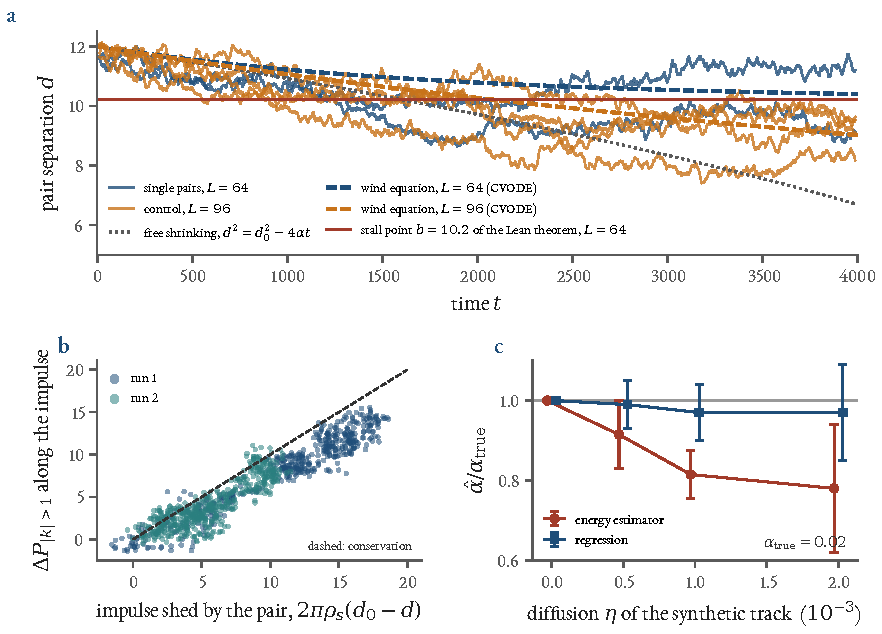
\includegraphics[width=\linewidth]{figures/ch07_failures.pdf}
\caption[Two theorems that were true and did not describe what they were applied to]{Two theorems that were true and did not describe what they were applied to. \textbf{a}~Separation of single pairs at $L=64$ (blue, two runs) and in the $L=96$ control (orange, four runs), $25$-unit running means, against the wind equation integrated with CVODE with the measured $\alpha=0.0062$ and no free parameter (thick dashed), free shrinking (dotted)
and the stall point $b$ of the Lean theorem (red). \textbf{b}~The wind seen directly: momentum of the phonon band $|k|>1$ projected on the initial impulse against the impulse shed by the pair, for the two $L=64$ runs; dashed, conservation of momentum between the pair and the phonons. \textbf{c}~The energy estimator of $\alpha$ on synthetic tracks of known $\alpha=0.02$ against the
diffusion $\eta$ of the track: exact at $\eta=0$ (the theorem), biased low when $\eta>0$; the regression estimator is not.}
\label{ch07:fig-failures}
\end{figure}

Then the control that the programme had registered as decisive was run. In an $L=96$ box at the same temperature ($\rho_n/\rho=0.029$) the same pair has $wd_0^2=3.2<4$: the equation has no zero (\Lthm{DissipativePairs}{wind_no_zero}), the box criterion $\rho_nL^2/(2\pi\rho_s)=44.3$ exceeds $d_0^2/4=36$, and no stall is predicted. A pair that keeps shrinking supports the mechanism; a pair that stalls near the $L=64$
separation refutes it. With a tie-break of two further runs written in advance, the four runs ended at $d=9.3,\ 9.6,\ 8.3,\ 9.5$ (wind equation: $8.0$--$8.9$; free shrinking: $5.3$--$6.5$), and the late shrinking rate was $0$, $10$ and $37\%$ of the early one in runs 2--4, where the mechanism predicted about $50\%$. Only one of four meets the no-stall criterion, and the rule (at most one: refuted) gives the verdict:
\textbf{W2 is refuted; the pairs stall at $L=96$ as at $L=64$, the stall is not the box's, and the explanation by the phonon wind of a closed box is withdrawn.} The parameter-free wind curve of \cref{ch07:fig-failures}a shows that a drift of the normal component is \emph{consistent} with the data (all six pairs end within 0.2--1.5 of the curve of their box, and 1.6 to 4.6 above free shrinking); consistent is not causal. The observation is kept (a reproducible, bath-driven stall
of a single pair at low temperature, with a $1/f^{0.5}$ separation spectrum), the explanation is not, and the graded test that could separate a residual wind from the real cause, a stall map in $L$, $d_0$ and $T$, is registered and has not been run. Every friction measurement on a single pair in a closed box at low temperature is affected, which is why the production runs use the zero-impulse geometry.

This is a clean example of what a proof assistant does and does not do. Lean certified the \emph{implication}: if the pair obeys the wind equation it cannot fall below $b$, and for $L=96$ the equation has no zero. The experiment tested the \emph{premise}, that the equation describes the pair, and refuted it. Nothing in the kernel could have said so.

\section{An estimator that was exact, and was not}\label{ch07:bias}

A second implementation is an instrument. The registered estimators were ported to Rust (crate \texttt{qf-pgpe}, module \texttt{transport}), first for speed, and the port agrees with the Python code on real tracks to $1\times10^{-14}$ (\cref{ch07:field}). Run on the registered synthetic gate G0 (known $\alpha=0.02$, $\alpha'=0.10$, $\eta=2\times10^{-3}$, eight tracks of $2000$ time units) over \emph{many seeds}, it showed what the single seed of
the gate had not.

With no diffusion the energy estimator returns the true value, exactly. With diffusion it is low, by $8.5$, $18.5$ and $22\%$ at $\eta=5\times10^{-4}$, $10^{-3}$, $2\times10^{-3}$, while the regression estimator is low by only $1$ to $3\%$ (\cref{ch07:fig-failures}c). The means over 8 seeds of eight tracks each are $0.0183\pm0.0017$, $0.0163\pm0.0012$, $0.0156\pm0.0032$ for the energy estimator and $0.0198\pm0.0012$, $0.0194\pm0.0014$, $0.0194\pm0.0024$ for the regression estimator, for a true $\alpha=0.02$ and no detection noise (Rust example \texttt{g0\_scan --eta-scan} of \texttt{qf-pgpe}, run for this chapter); the ledger records the bias as independent of the detection noise (CLAIM-098). The gate's criterion (energy estimator within $15\%$) passes on $2$ of $12$ seeds (CLAIM-098); the registered gate had
passed on one lucky seed. In the real arms the regression estimator exceeds the energy one by $5$ to $21\%$, in exactly this direction.

Why did the theorem not warn us? Because it is not about this. Its hypothesis is \texttt{hr}: the path has a derivative at every instant and obeys the flow (\Lthm{DissipativeVortexDynamics}{energy_dissipation}). A diffusing vortex has no derivative; the identity belongs to the \emph{deterministic} model, and the data are not a path of that model. The cause of the bias is not proven (the programme's note suspects that the stochastic part of $H(t)$ is
correlated with the cumulative regressor $\int2S\,dt$, which depends on the same noisy path); what is proven is that the identity applies where its hypothesis holds, and there it is exact ($\alpha_{\rm energy}=0.0200$ at $\eta=0$). This is LL-15 applied to the programme's own tool: a conclusion travels with its preconditions or not at all. No registered verdict changes (they compare arms with the same estimator), but the absolute $\alpha$ of \cref{ch07:tab-alpha}
are low by about $5$--$20\%$ ($0.0062$, $0.014$, $0.02$ become $0.0064$, $0.0156$, $0.0242$ with the regression estimator, \cref{ch07:tab-alpha}), the temperature law reads $0.060\,T$ rather than $0.054\,T$, and the gate's energy criterion is not a reliable known answer; the regression criterion is.

\section{What this chapter establishes, and what it does not}\label{ch07:honest}

\begin{honestbox}
\textbf{Proved in Lean (standard axioms only; checked on 2026-10-09).} The energy identity for any flow of the form~\eqref{ch07:eq-flow}; for the plane dipole, the law $|\mathbf d|^2=|\mathbf d_0|^2-4\alpha t$ and the centre velocity $(1-\alpha')/|\mathbf d|$, and, in the book's new module, the law $+4\alpha t$ of the same-sign pair; the zero-current characterisation $DK=2\alpha$; the kinetic identity for $\alpha/(\rho_n/\rho)$; the stall of the wind equation and, new, its stall at the root $b$; the bound on quasi-periodic mean-square displacements (\cref{ch07:lean,ch07:law,ch07:alphaprime,ch07:wind}). These are statements about \emph{models}, elementary and not new (the new theorems are in \texttt{book/lean/}, not in the library), and none is a statement of Godfrin's papers.

\textbf{Simulated, in a classical projected field (one box, $mg=1$, cutoffs $2\pi/3$, $\pi$, $2\pi$, $T<0.45\,T_{\rm BKT}$).} $\alpha=0.0062(4)$, $0.014(2)$, $0.02(1)$ at $T/T_{\rm BKT}=0.14$, $0.27$, $0.43$ by two estimators, the energy one low by $5$--$20\%$; $\alpha\simeq0.054\,T$ (energy) or $0.060\,T$ (regression) over three cutoffs; $\alpha'=0$ within about $1\%$ once the $T=0$ kinematics of a compressible pair on a torus are
accounted for; the diffusion $1.4$--$3$ times the Einstein value where it can be read; a bath-driven stall of a single pair; one fresh run of $1500$ time units, one seed, inside the scatter of single runs. CVODE reproduces the exact pair laws to $3\times10^{-8}$ (dipole) and $10^{-5}$ (rotating pair).

\textbf{Analogy only, not established.} Anything about helium, atomic gases, or the fluid whose excitations Godfrin measured: the classical-field bath is not a Bose bath (\cref{ch07:law}), the temperature of the field is a parameter of the model, and $\sigma_{\rm tr}(k)$ of a vortex has not been measured here. The Einstein relation is undecided by the registered rule.

\textbf{Failed, withdrawn or corrected.} The first known-answer gate passed on a defective imprint and is withdrawn (CLAIM-075). The reading $\alpha\propto\rho_n$ with a vortex-owned coefficient and the ``geometric core size'' $1.4\xi$ are withdrawn: the coefficient depends on the cutoff, and the registered predictions of FL2 and of the Born law failed. The registered Iordanskii-like prediction for $\alpha'$ is refuted at $18\sigma$. The phonon-wind mechanism is
refuted by the $L=96$ control while its Lean theorem stays true. The energy estimator is biased low by the diffusion, which no theorem was about. The temperature law was formulated after the data of five arms were read and is confirmed, by the registered window, on a sixth arm whose error is larger than was assumed.
\end{honestbox}

\section{Exercises}

\paragraph{Exercise 1.} Show that two vortices of the \emph{same} sign obey $|\mathbf d|^2=|\mathbf d_0|^2+4\alpha t$ and rotate with angular velocity $2(1-\alpha')/|\mathbf d|^2$ about their fixed centre, and find how long a pair with $d_0=4\xi$ and $\alpha=0.02$ takes to double its separation. Then reproduce panel~b of \cref{ch07:fig-dipole}: the listing of \cref{ch07:cvode} needs only a new right-hand side, for two vortices of the same sign.
\emph{Hint.} With $\mathbf d=\mathbf p_1-\mathbf p_2$ the velocities induced at the two vortices are $\pm\hat{\mathbf z}\times\mathbf d/|\mathbf d|^2$; the radial component of $\dot{\mathbf d}$ is $2\alpha/d$, so $d\,\dot d=2\alpha$; the answer to the first question is $3d_0^2/(4\alpha)=600$.

\paragraph{Exercise 2.} Generate synthetic dipole tracks with the Langevin generator of the repository (\texttt{exploration/pgpe/transport\_estimators.py}, function \texttt{langevin}) for $\alpha=0.02$ and $\eta=0$, then $\eta=10^{-3}$, and apply the energy and the regression estimators through \texttt{qf\_pgpe.analyse\_tracks}. Explain, from the hypotheses of \Lthm{DissipativeVortexDynamics}{energy_dissipation}, why the first case must be exact and why
the second need not be. \emph{Hint.} Look at \texttt{hr}: what regularity does a Brownian path have? Expect $\alpha_{\rm energy}\approx0.016$ at $\eta=10^{-3}$ over eight tracks of $2000$ time units.

\paragraph{Exercise 3.} (LL-15.) For $\varepsilon_k=\sqrt{k^2+k^4/4}$ at $T=0.115$ compute $n_{\rm RJ}/n_{\rm Bose}$, with $n_{\rm RJ}=T/\varepsilon_k$ and $n_{\rm Bose}=1/(e^{\varepsilon_k/T}-1)$, at $k=0.2,\,1,\,\pi$. Then compute the fraction of the equipartition Landau sum $\tfrac12L^{-2}\sum_kk^2T/\varepsilon_k^2$ carried by modes with $\varepsilon<T$, on the $3208$ modes of the disk $|k|\le\pi$,
$L=64$. Which statements of \cref{ch07:law} depend on the equipartition occupation, and which would survive in a Bose bath? \emph{Hint.} The first part is three lines of code; the second is a fraction of a per cent.

\section{Notes and further reading}

The programme's two papers on the subject are \cite{Callens2026a}, on friction, the transverse coefficient, the diffusion and the stall of a single pair (Zenodo, version~2.2, October 2026, \texttt{doi:10.5281/\allowbreak zenodo.23262143}), and \cite{Callens2026b}, on the cutoff scan and the temperature law (\texttt{doi:10.5281/\allowbreak zenodo.23262132}); the engine is in \cite{Callens2026sw}, the Lean library in \cite{Callens2026lib}. The static half of the first paper, the box-scale pair, equilibration and the polarisability
of the pair gas, bears on the Kosterlitz--Thouless side of \cref{ch06} and is not treated here. For mutual friction in helium start with Donnelly's book~\cite{Donnelly1991} and the review of Sergeev~\cite{Sergeev2023}; for measurements in atomic gases, \cite{Moon2015} and \cite{Neely2024}, and, in a Fermi superfluid, where the friction and the vortex Hall angle were measured, \cite{Grani2025}; for the diffusion, \cite{Mehdi2023}, and for the stochastic point-vortex model as used
for helium films, \cite{AHNS1980}; for the transverse force, \cite{ThoulessAoNiu1996}, \cite{Iordanskii1964} and \cite{Sonin1997}. The point-vortex flow on the torus is in \cite{WeissMcWilliams1991}, and the integrability of few-vortex flows in the survey~\cite{ModinViviani2021}.
\widowpenalty=\chsevenwp\relax\clubpenalty=\chsevencp\relax
\flushbottom
